\documentclass{article}
\usepackage[utf8]{inputenc}
\usepackage{amsmath}
\usepackage{systeme}
\usepackage{amssymb}
\usepackage[most]{tcolorbox}
\usepackage[scale=.95,type1]{cabin}
\usepackage{lmodern}
\usepackage{enumitem}

\usepackage{float}
\usepackage{graphicx}

\usepackage[legalpaper,margin=1in]{geometry}

\setlength{\parindent}{10pt}
\setlength{\parskip}{1em}
\renewcommand{\baselinestretch}{1.2}

\title{Applications of Inner Product Spaces}
\date{}

\newcounter{example}[section]
\newenvironment{example}[1][]{\refstepcounter{example}\par\medskip
   \noindent \textbf{Example~\theexample. #1} \rmfamily}{\medskip}

\makeatletter
\renewcommand*\env@matrix[1][*\c@MaxMatrixCols c]{%
  \hskip -\arraycolsep
  \let\@ifnextchar\new@ifnextchar
  \array{#1}}
\makeatother

\newcommand\y{\cellcolor{blue!10}}
\newcommand\B{\textbf}
\newcommand\tcl{\begin{tcolorbox}[colback = {blue9}]}
\newcommand\etcl{\end{tcolorbox}}

\usepackage{tabularray}
\SetTblrInner{colsep=5pt,rowsep=1pt}

\newcommand\x{\times}
\newcommand\xor{\oplus}

\makeatletter
\newcommand{\dashover}[2][\mathop]{#1{\mathpalette\df@over{{\dashfill}{#2}}}}
\newcommand{\fillover}[2][\mathop]{#1{\mathpalette\df@over{{\solidfill}{#2}}}}
\newcommand{\df@over}[2]{\df@@over#1#2}
\newcommand\df@@over[3]{%
  \vbox{
    \offinterlineskip
    \ialign{##\cr
      #2{#1}\cr
      \noalign{\kern1pt}
      $\m@th#1#3$\cr
    }
  }%
}
\newcommand{\dashfill}[1]{%
  \kern-.5pt
  \xleaders\hbox{\kern.5pt\vrule height.4pt width \dash@width{#1}\kern.5pt}\hfill
  \kern-.5pt
}
\newcommand{\dash@width}[1]{%
  \ifx#1\displaystyle
    2pt
  \else
    \ifx#1\textstyle
      1.5pt
    \else
      \ifx#1\scriptstyle
        1.25pt
      \else
        \ifx#1\scriptscriptstyle
          1pt
        \fi
      \fi
    \fi
  \fi
}
\newcommand{\solidfill}[1]{\leaders\hrule\hfill}
\makeatother

\newcommand\R{\mathbb{R}}
\newcommand\T{\textit}
\usepackage{mathtools}

\DeclarePairedDelimiter\abs{\lvert}{\rvert}%
\DeclarePairedDelimiter\norm{\lVert}{\rVert}%

% Swap the definition of \abs* and \norm*, so that \abs
% and \norm resizes the size of the brackets, and the 
% starred version does not.
\makeatletter
\let\oldabs\abs
\def\abs{\@ifstar{\oldabs}{\oldabs*}}
%
\let\oldnorm\norm
\def\norm{\@ifstar{\oldnorm}{\oldnorm*}}
\makeatother

\newcommand*{\Value}{\frac{1}{2}x^2}%
\newcommand\la{\langle}
\newcommand\ra{\rangle}
\newcommand\ddfrac[2]{\frac{\displaystyle #1}{\displaystyle #2}}


\begin{document}
    \section{The Cross Product of Two Vectors in Space}
    Here we will look at a vector product that yields a vector in $\R^3$ orthogonal to 2 vectors. This vector product is
    called the \textbf{cross product}, and it is defined and calculated with standard unit vectors
    \[ \B{v} = (v_1, v_2, v_3) = v_1\B{i} + v_2\B{j} + v_3\B{k} \]
    \begin{tcolorbox}[colback = {blue9}]
        \textbf{Definition of Cross Product of Two Vectors.}

        Let $\B{u} = u_1\B{i} + u_2\B{j} + u_3\B{k}$ and $\B{v} = v_1\B{i} + v_2\B{j} + v_3\B{k}$ be vectors in $\R^3$. The \textbf{cross product}
        of \textbf{u} and \textbf{v} is the vector
        \[\B{u} \times \B{v} = (u_2v_3 - u_3v_2)\B{i} - (u_1v_3 - u_3v_1)\B{j} + (u_1v_2 - u_2v_1)\B{k}\]        

    \textbf{Alternative form of the Cross Product}
    \[ \B{u} \times \B{v} = 
        \begin{vmatrix}
            \B{i} & \B{j} & \B{k} \\
            u_1 & u_2 & u_3 \\
            v_1 & v_2 & v_3
        \end{vmatrix} \]
    \end{tcolorbox}
    \textbf{Example. \textcolor{blue5}{Finding the Cross Product of Two Vectors}}

    Provided that $\B{u} = \B{i} - 2\B{j} + \B{k}$ and $\B{v} = 3\B{i} + \B{j} - 2\B{k}$. 

    (a) \begin{equation*}
        \begin{split}
            \B{u} \x \B{v} & =         \begin{vmatrix}
            \B{i} & \B{j} & \B{k} \\
            1 & -2 & 1 \\
            3 & 1 & -2
        \end{vmatrix}  \\
                           & = 3\B{i} + 5\B{j} + 7\B{k}
        \end{split}
    \end{equation*}
    (b) $\B{v} \times \B{u} = -3\B{i} - 5\B{j} - 7\B{k}$
    
    (c) $\B{v} \times \B{v} = \B{0}$
    
    Those results suggest some \textit{algebraic} properties of the cross product.
    \begin{tcolorbox}[colback = {blue9}]
        \textit{THEOREM 5.17} \textbf{Algebraic Properties of the Cross Product}

        If \B{u}, \B{v} and \B{w} are vectors in $\R^3$, and $c$ is a scalar, then the following properties are true.
        \begin{enumerate}[itemsep=0mm]
            \item $\B{u} \times \B{v} = -(\B{v} \times \B{u})$
            \item $\B{u} \times (\B{v} + \B{w} = (\B{u} \times \B{v}) + (\B{u} \times \B{w})$
            \item $c(\B{u} \times \B{v}) = c\B{u} \times \B{v} = \B{u} \times c\B{v}$
            \item $\B{u} \times \B{0} = \B{0} \times \B{u} = \B{0}$
            \item $\B{u} \times \B{u} = \B{0}$
            \item $\B{u} \cdot (\B{v} \times \B{w}) = (\B{u} \times \B{v}) \cdot \B{w}$
        \end{enumerate}
    \end{tcolorbox}
    \textbf{Note.} $\B{u} \times \B{v}$ and $\B{v} \times \B{u}$ have equal lengths but \textit{opposite direction}.

    %\vspace{5mm} %5mm vertical space
            \begin{tcolorbox}[colback = {blue9}]

            \textit{THEOREM 5.18} 
            \textbf{Geometric Properties of the Cross Product}

            If \B{u} and \B{v} are nonzero vectors in $\R^3$, then the following properties are true.
            \begin{enumerate}[itemsep=0mm]
                \item $\B{u} \times \B{v}$ is orthogonal to both \textbf{u} and \textbf{v}.
                \item The angle $\theta$ between \B{u} and \B{v} is given by
                    \[\norm{\B{u} \times \B{v}} = \norm{\B{u}} \norm{\B{v}} \sin{\theta} \]
                \item \B{u} and \B{v} are parallel if and only if $\B{u} \times \B{v} = 0$.
                \item The \textit{parallelogram} having \B{u} and \B{v} as adjacent sides has an area of $\norm{\B{u} \times \B{v}}$.
            \end{enumerate}
        \end{tcolorbox} 
    
        \begin{minipage}{0.15\linewidth}
            \textit{ \textcolor{blue5}{PROOF.} }        
        \end{minipage}
        \begin{minipage}{0.5\linewidth}
            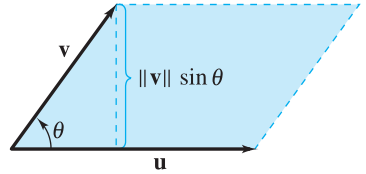
\includegraphics[width = 5cm] {images/uvsin.png}
        \end{minipage}

        \textbf{Note.} The 3 vectors \textbf{u}, \textbf{v}, and $\B{u} \times \B{v}$ form a \textit{right-handed system}, whereas the 3 vectors
        \textbf{u}, \textbf{v} and $\B{u} \times \B{v}$ form a \textit{left-handed system}.
        \begin{center}
            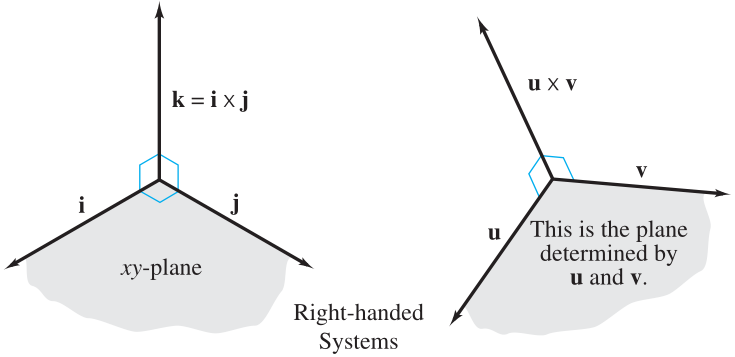
\includegraphics[width = 10cm]{images/righthanded.png}
        \end{center}
    
    \section{Least Square Approximations (Calculus)}
    Many problems in the physical sciences and engineering involve an approximation of a function $f$ by another function $g$.
    If $f$ is in $C[a,b]$ (the inner product space of all continuous funtions on $[a,b]$), then $g$ is usually chosen from a
    subspace $W$ of $C[a,b]$.

    For instance, to approximate the function 
    \[f(x) = e^x, \quad 0 \le x \le 1,\]
    you could choose one of the following forms of $g$.

    \begin{minipage}{0.5\linewidth}
            1. $g(x) = a_0 + a_1x, \quad 0 \le x \le 1$

            2. $g(x) = a_0 + a_1x + a_2x^3, \quad 0 \le x \le 1$

            3. $g(x) = a_0 + a_1\cos{x} + a_2\sin{x}, \quad 0 \le x \le 1$
    \end{minipage}
    \begin{minipage}{0.3\linewidth}
        \linespread{2.0}
            {\footnotesize \textcolor{blue5}{Linear}}

            {\footnotesize \textcolor{blue5}{Quadratic}}

            {\footnotesize \textcolor{blue5}{Trigonometric}}
    \end{minipage}

    Before discussing ways of finding $g$, we must define how 1 function can "best" approximate another. One natural way would
    require the area bounded by the graphs of $f$ and $g$ on the interval $[a,b]$.

    \begin{minipage}{0.5\linewidth}
    \[\text{Area} = \int_a^b |f(x) - g(x)|\,dx,\]
    to be a minimum with respect to other functions in the subspace $W$
        
    \end{minipage}
    \begin{minipage}{0.45\linewidth}
        \begin{flushright}
            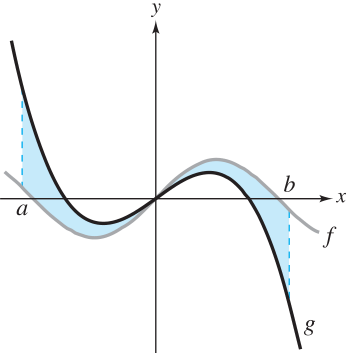
\includegraphics[width = 5.5cm]{images/intfg.png}
        \end{flushright}
    \end{minipage}

    Integrands involving absolute value are difficult to evaluate, so it is more common to \textbf{square} the integrand.
    \begin{tcolorbox}[colback = {blue9}]
        \textbf{Definition of Least Squares Approximation}

        Let $f$ be continuous on $[a,b]$, and $W$ be a subspace of $C[a,b]$. A function $g$ in $W$ is called a \textbf{least squares
        approximation} of $f$ with respect to $W$ if the value of 
        \[I = \int_a^b [f(x) - g(x)]^2\,dx\]
        is a minimum with respect to all other functions in $W$.

    \end{tcolorbox}
    \textbf{REMARK.} If the subspace $W$ is the entire space $C[a,b]$, then $g(x) = f(x)$, which implies that $I = 0$.

    \textbf{Example 4. \textcolor{blue5}{Finding a Least Squares Approximation}}

    Find the least squares approximation $f(x) = a_0 + a_1x$ for
    \[f(x) = e^x, \quad 0 \le  x \le 1\]
    \textit{ \textcolor{blue5}{SOLUTION.} } For this approximation, we need to find the constant $a_0$ and $a_1$ that minimize
    the value of
    \begin{equation*}
        \begin{split}
            I &= \int_0^1 [f(x) - g(x)]^2\,dx \\
              &= \int_0^1 (e^x - a_0 - a_1x)^2\,dx
        \end{split}
    \end{equation*}
    Evaluating this integral, you have
    \begin{equation*}
        \begin{split}
            I &= \int_0^1 (e^x - a_0 - a_1x)^2\,dx\\
              &= \int_0^1 (e^{2x} - 2a_0e^x - 2a_1xe^x + a_0^2 + 2a_0a_1x + a_1x^2)\,dx\\
              &= \left[ \frac{1}{2}e^{2x} - 2a_0e^x - 2a_1e^x(x - 1) + a_0^2x + a_0a_1x^2 + a_1^2\frac{x^3}{3} \right]_0^1 \\
              &= \frac{1}{2}(e^2 - 1) - 2a_0(e - 1) - 2a_1 + a_0^2 + a_0a_1 + \frac{1}{3}a_1^2
        \end{split}
    \end{equation*}
    Now, considering $I$ to be a function of the variables $a_0$ and $a _{1}$, use calculus to determine their values to
    minimize $I$. Specifically, by setting the partial derivatives
    \begin{equation*}
        \begin{split}
            \ddfrac{\partial I}{\partial a_0} &= 2a_0 - 2e + 2 + a_1 \\
            \ddfrac{\partial I}{\partial a_1} &= a_0 + \ddfrac{2}{3}a_1 - 2
        \end{split}
    \end{equation*}
    equal to zero, we obtain the following 2 linear equations in $a_0$ and $a_1$ 
    \[\systeme {
        2a_0 + a_1 = 2(e - 1),
        3a_0 + 2a_1 = 6
    }, \text{which solution is}
    \begin{cases}{}
        a_0 = 4e - 10 \approx 0.873 \\
        a_1 = 18 - 6e \approx 1.690
    \end{cases}
    \]

    \begin{minipage}{0.3\linewidth}
        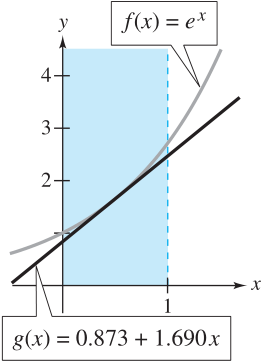
\includegraphics[width = 4cm]{images/ansint1.png}
    \end{minipage}
    \begin{minipage}{0.6\linewidth}
        So, the best \textit{linear approximation} of $f(x) = e^x$ on the interval $[0,1]$ is
        \begin{equation*}
            \begin{split}
                g(x) &= 4e - 10 + (18 - 6e)x \\
                     &\approx 0.873 + 1.690x
            \end{split}
        \end{equation*}
    \end{minipage}

    Of course, the approximation obtained depends on the \textit{definition of the best approximation}. If that 
    definition of "best" had been the \textit{Taylor polynomial of degree 1} centered at 0.5, $g$ would have been
    \begin{equation*}
        \begin{split}
            g(x) &= f(0.5) + f'(0.5)(x - 0.5) \\
                 &= e^{0.5} + e^{0.5}(x - 0.5) \\
                 &\approx 0.824 + 1.649x
        \end{split}
    \end{equation*}
    \textbf{Example 5. \textcolor{blue5}{Finding a Least Squares Approximation}}

    Find the least squares approximation $f(x) = a_0 + a_1x + a_2x^2$ for
    \[f(x) = e^x, \quad 0 \le x \le 1\]
    \textit{ \textcolor{blue5}{SOLUTION.} } We need to find the values of $a_0, a_1$ and $a_2$ that minimize the value of
    \begin{equation*}
        \begin{split}
            I =& \int_0^1 [f(x) - g(x)]^2\,dx \\
            =& \int_0^1 (e^x - a_0 - a_1x - a_2x^2)^2\,dx \\
            =& \ddfrac{1}{2}(e^2 - 1) + 2a_0(1 - e) + 2a_2(2 - e)\\
             & + a_0^2 + a_0a_1 + \ddfrac{2}{3}a_0a_2 + \ddfrac{1}{2}a_1a_2 + \ddfrac{1}{3}a_1^2 + 
             \ddfrac{1}{5}a_2^2 - 2a_1
        \end{split}
    \end{equation*}
    Integrating and then setting the partial derivatives of $I$ (with respect to $a_0, a_1$ and $a_2$) equal to zero produces
    the following system of linear equations.
    \[ \systeme {
            6a_0 + 3a_1 + 2a_2 = 6(e - 1),
            6a_0 + 4a_1 + 3a_2 = 12,
            20a_0 + 15a_1 + 12a_2 = 60(e - 2)
        } \]
        The solution of this system is $\begin{cases}
            a_0 = -105 + 39e \approx 1.013 \\
            a_1 = 588 - 216e \approx 0.851 \\
            a_2 = -570 + 210e \approx 0.839
      \end{cases}$

      \begin{minipage}{0.6\linewidth}
          So, the approximating function $g$ is
          \[g(x) \approx 1.013 + 0.851x + 0.839x^2\]
      \end{minipage}
      \begin{minipage}{0.3\linewidth}
          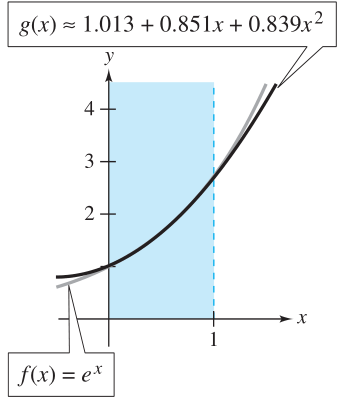
\includegraphics[width = 4cm]{images/ansint2.png}
      \end{minipage}\\
    {\color{blue9} \rule{5cm}{0.3mm}}\\
    The integral $I$ can be expressed in vector form. First, use the \textbf{inner product}
    \begin{equation*}
        \begin{split}
            \la f, g \ra &= \int_a^b f(x)g(x)\,dx \\
            \text{With this, we have: } \qquad I &= \int_a^b [f(x) - g(x)]^2\,dx = \la f - g, f - g \ra = \norm{f - g}^2
        \end{split}
    \end{equation*}
    In other words, $g \in W$ is \textit{closest} to $f$ in term of the inner product $\la f, g \ra$.
    \begin{tcolorbox}[colback = {blue9}]
        \textit{THEOREM 5.19} \textbf{Least Squares Approximation}

        Let $f$ be continuous on $[a, b]$, $W$ be a finite-dimensional subspace of $C[a,b]$. \\
        The least squares approximating function of $f$ with respect to $W$ is given by
        \[g = \la f, \B{w}_1 \ra \B{w}_1 + \la f, \B{w}_2 \ra \B{w}_2 + \cdots + \la f, \B{w}_n \ra \B{w}_n,\]
        where $B = \{ \B{w}_1, \B{w}_2, \dots, \B{w}_n \}$ is an \textit{orthornormal} basis for $W$.
    \end{tcolorbox}
    %{\color{blue9} \rule{5cm}{0.3mm}}
    Now observe how this can be used to produces least squares approximation obtained in \textbf{Example 4.}

    First, apply the Gram-Schmidt orthornormalization process to the standard basis $B = \{1, x^2\}$ of $W$
    to obtain the orthornormal basis $B = \{1, \sqrt{3}(2x - 1) \}$. Then we got
    \begin{equation*}
        \begin{split}
            g(x) &= \la e^x, 1 \ra(1) + \la e^x, \sqrt{3}(2x - 1) \ra \sqrt{3}(2x - 1) \\
                 &= \int_0^1 e^x\,dx + \sqrt{3}(2x - 1)\int_0^1 \sqrt{3}e^x(2x - 1)\,dx \\
                 &= \int_0^1 e^x\,dx + 3(2x - 1)\int_0^1 e^x(2x - 1)\,dx \\
                 &= (e - 1) + 3(2x - 1)(3 - e) \\
                 &= 4e - 10 + (18 - 6e)x
        \end{split}
    \end{equation*}
    which agrees with the result obtained in \textbf{Example 4}.

    \textbf{Example 6. \textcolor{blue5}{Finding a Least Squares Approximation}}

    Find the least squares approximation for $f(x) = \sin{x}, \quad 0 \le x \le \pi,$ with respect to the subspace $W$
    of quadratic functions.

    \textit{ \textcolor{blue5}{SOLUTION.} } Applying the Gram-Schmidt orthonormalization process to the standard
    basis for $W$, $\{1, x, x^2 \}$, obtaining the orthornormal basis
    \begin{equation*}
        \begin{split}
            B &= \{ \B{w}_1, \B{w}_2, \B{w}_3 \}\\
              &= \left\{ \ddfrac{1}{\sqrt{\pi}}, \ddfrac{\sqrt{3}}{\pi\sqrt{\pi}}(2x - \pi), \ddfrac{\sqrt{5}}{\pi^2\sqrt{\pi}}(6x^2 - 6\pi x + \pi^2) \right\}
        \end{split}
    \end{equation*}
    The least squares approximating function $g$ is 
    \[g(x) = \la f, \B{w}_1 \ra \B{w}_1 + \la f, \B{w}_2 \ra \B{w}_2 + \la f, \B{w}_3 \ra \B{w}_3 \]
    and we have
    \begin{equation*}
        \begin{split}
            \la f, \B{w}_1 \ra &= \ddfrac{1}{\sqrt{\pi}} \int_0^\pi \sin{x}\,dx = \ddfrac{2}{\sqrt{\pi}} \\
            \la f, \B{w}_2 \ra &= \ddfrac{\sqrt{3}}{\pi\sqrt{\pi}} \int_0^\pi \sin{x}(2x - \pi)\,dx = 0 \\
            \la f, \B{w}_3 \ra &= \ddfrac{\sqrt{5}}{\pi^2\sqrt{\pi}}\int_0^\pi \sin{x}(6x^2 - 6\pi x + \pi^2)\,dx \\
                              &= \ddfrac{2\sqrt{5}}{\pi^2\sqrt{\pi}}(\pi^2 - 12)
        \end{split}
    \end{equation*}
    \begin{minipage}{0.3\linewidth}
        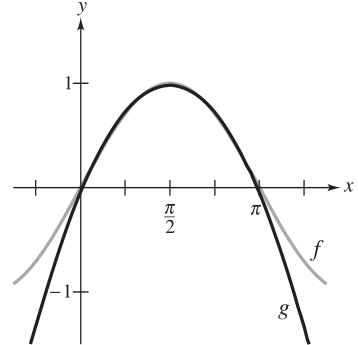
\includegraphics[width = 4cm]{images/integ6.png}
    \end{minipage}
    \begin{minipage}{0.6\linewidth}
        So, $g$ is
        \begin{equation*}
            \begin{split}
                g(x) &= \ddfrac{2}{\pi} + \ddfrac{10(\pi^2 - 12)}{\pi^5}(6x^2 - 6\pi x + \pi^2) \\
                     &\approx -0.4177x^2 + 1.3122x - 0.0505
            \end{split}
        \end{equation*}
    \end{minipage}

    \section{Fourier Approximations (Calculus)}
    We will now look at a special type of least squares approximation called a \textbf{Fourier approximation}. For this 
    approximation, consider functions of the form
    \[g(x) = \ddfrac{a_0}{2} + a_1\cos{x} + \cdots + a_n\cos{nx} + b_1\sin{x} + \cdots + b_n\sin{nx} \]
    in the subspace $W$ of $C[0, 2\pi]$ spanned by the basis
    \[S = \{1, \cos{x}, \cos{2x}, \dots, \cos{nx}, \sin{x}, \sin{2x}, \dots , \sin{nx} \} \]
    These $2n + 1$ vectors are \textit{orthogonal} in the inner product space $C[0, 2\pi]$ because
    \[\la f, g \ra = \int_0^{2\pi} f(x)g(x)\,dx = 0, f \ne g, \]
    Moreover, by normalizing each function in this basis, we obtain the orthonormal basis
    \[B = \left\{ \ddfrac{1}{\sqrt{2\pi}}, \ddfrac{1}{\sqrt{\pi}} \cos{x}, \dots, \ddfrac{1}{\sqrt{\pi}} \cos{nx}, \ddfrac{1}{\sqrt{\pi}} \sin{x}, \dots, \ddfrac{1}{\sqrt{\pi}} \sin{nx}\right\} \]
    With this orthonormal basis, we can apply Theorem 5.19 to write
    \[g(x) = \la f, \B{w}_0 \ra \B{w}_0 + \la f, \B{w}_1 \ra \B{w}_1 + \cdots + \la f, \B{w}_{2n} \ra \B{w}_{2n},\]
    It will now called the \textbf{$n$th-order Fourier approximation} of $f$ on the interval $[0, 2\pi]$.
    \begin{tcolorbox}[colback = {blue9}]
        \textit{THEOREM 5.20} \textbf{Fourier Approximation}

        On the interval $[0, 2\pi]$, the least squares approximation of a continuous function $f$ with respect
        to the vector space spanned by $ \{1, \cos{x}, \cos{2x}, \dots, \cos{nx}, \sin{x}, \sin{2x}, \dots , \sin{nx} \}$ is
        given by
            \[g(x) = \ddfrac{a_0}{2} + a_1\cos{x} + \cdots + a_n\cos{nx} + b_1\sin{x} + \cdots + b_n\sin{nx} \]
        where the \textbf{Fourier coefficients} $a_0, a_1, \dots, a_n, b_1, \dots, b_n$ are
        \begin{equation*}
            \begin{split}
                a_0 &= \ddfrac{1}{\pi}\int_0^{2\pi} f(x)\,dx \\
                a_j &= \ddfrac{1}{\pi}\int_0^{2\pi} f(x) \cos{jx}, \quad j = 1, 2, \dots, n\\
                b_j &=  \ddfrac{1}{\pi}\int_0^{2\pi} f(x) \sin{jx}, \quad j = 1, 2, \dots, n
            \end{split}
        \end{equation*}
    \end{tcolorbox}
    \pagebreak
    \textbf{Example 7. \textcolor{blue5}{Finding a Fourier Approximation}}

    Find the third-order approximation of $f(x) = x, 0 \le x \le 2\pi$.\\
    \textit{ \textcolor{blue5}{SOLUTION.} } Using Theorem 5.20, we have
    \[g(x) = \ddfrac{a_0}{2} + a_1 \cos{x} + a_2 \cos{2x} + a_3 \cos{3x} + b_1 \sin{x} + b_2 \sin{2x} + b_3 \sin{3x}\]
    where 
    \begin{equation*}
        \begin{split}
            a_0 &= \ddfrac{1}{\pi}\int_0^{2\pi} x\,dx = \ddfrac{1}{\pi} 2\pi^2 = 2\pi \\
            a_j &= \ddfrac{1}{\pi}\int_0^{2\pi} x \cos{jx} = \left[ \ddfrac{1}{\pi j^2} \cos{jx} + \ddfrac{x}{\pi j} \sin{jx} \right]_0^{2\pi} = 0\\
            b_j &=  \ddfrac{1}{\pi}\int_0^{2\pi} x \sin{jx} =  \left[ \ddfrac{1}{\pi j^2} \sin{jx} + \ddfrac{x}{\pi j} \cos{jx} \right]_0^{2\pi} =  -\ddfrac{2}{j}
        \end{split}
    \end{equation*}
    \begin{minipage}{0.31\linewidth}
        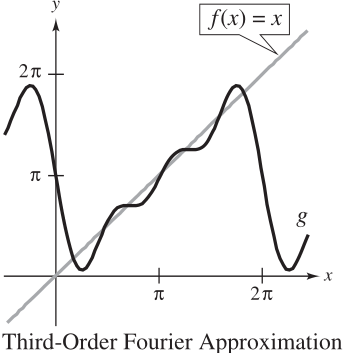
\includegraphics[width = 4cm]{images/3fourier.png}
    \end{minipage}
    \begin{minipage}{0.59\linewidth}
        So, we have 
        \begin{equation*}
            \begin{split}
                g(x) &= \ddfrac{2\pi}{2} - 2 \sin{x} - \sin{2x} - \ddfrac{2}{3} \sin{3x} \\
                     &= \pi - 2 \sin{x} - \sin{2x} - \ddfrac{2}{3} \sin{3x}
            \end{split}
        \end{equation*}
    \end{minipage}

    We've got a general pattern for the Fourier coefficients here. The $n$th-order Fourier approximation is
    \[g(x) = \pi - 2 \left( \sin{x} + \ddfrac{1}{2} \sin{2x} + \ddfrac{1}{3} \sin{3x} + \cdots + \ddfrac{1}{n} \sin{nx}  \right)\]
    As $n$ increases, the Fourier approximation improves.
    \begin{center}
        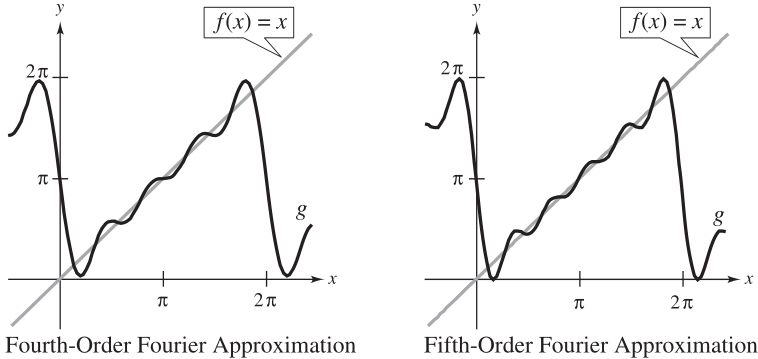
\includegraphics[width = 10cm]{images/45fourier.png}
    \end{center}
    In advanced courses, it is shown that as $n \to \infty$, the approximation error $\norm{f - g}$ approaches zero for
    all $x \in [0, 2\pi]$. The infinite \textit{series} for $g(x)$ is called a \textbf{Fourier series}.
    
    \textbf{Example 8. \textcolor{blue5}{Finding a Fourier Approximation}}

    Find the fourth-order Fourier approximation of $f(x) = |x - \pi|, 0 \le x \le 2\pi$.

    \begin{minipage}{0.6\linewidth}
       \textit{ \textcolor{blue5}{SOLUTION.} } Applying Theorem 5.20, find the Fourier coefficients and obtaining
        \[g(x) = \ddfrac{\pi}{2} + \ddfrac{4}{\pi} \cos{x} + \ddfrac{4}{9\pi} \cos{3x} \]

    \end{minipage}
    \begin{minipage}{0.3\linewidth}
        \begin{flushright}
            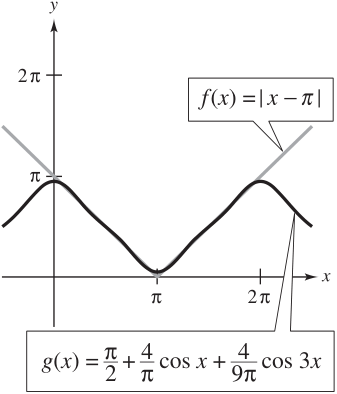
\includegraphics[width = 4cm]{images/8fourier.png}
        \end{flushright}
    \end{minipage}





\end{document}
